\chapter{Rolling Stock RFID Management}
\section{Introduction}
\gls{rails} is a software model and implementation of an automated system to assist the model railroader achieve realism in the operation of a model railroad.
The \gls{rails} system design describes the system's architecture, components, and interfaces and can be found at \href{https://github.com/djbristow/RAILS/blob/master/Documentation/rails-system.pdf}{RAILS System Design and implementation}.
There are four user interface \glspl{spa} that provide different aspects of \gls{rails} they are:
\begin{itemize}
  \item \gls{rsrm}, the focus of this manual, allows the user to:
	\begin{itemize}
		\item view rolling stock information associated with scanned \gls{rfid} tags;
		\item manually input rolling stock information when an \gls{rfid} tag is not recognized; and
		\item maintain a database of \gls{rs} and associated \gls{rfid} tags.
	\end{itemize}
  \item \gls{mrim} allows the user to create, update and delete model railroad assets, such as \gls{rs};
  \item \gls{mppm} allows the user to enter information about their projects and purchases; and
  \item \gls{mrlm} allows the user to enter information about their layout and control elements of it.
\end{itemize}
\section{Components}
The implementation of \gls{rsrm} consists of the following micro-services components:
\begin{itemize}
\item \gls{rfid} Controller is a micro-controller that processes \gls{rfid} tags obtained from a \gls{rfid} reader and then publishes \gls{iot} messages to the \gls{mqtt} Broker;
\item \gls{mqtt} Broker is responsible for receiving \gls{rfid} and micro info messages, filtering them, posting to designated topics and sending messages to clients subscribing to topics. 
The subscribers and publishers bridge the \gls{mqtt} elements with the GUI applications. The broker handles \gls{iot} messages;
\item \gls{isrs} subscribes to \gls{rfid} messages and pushes them via a web-socket to the RSRM component;
\item \gls{isms} that subscribes to micro controller startup and heartbeat messages, updating the micros collection via \gls{rlds};
\item \gls{rlds} provides \gls{rest} access to model railroad layout collections including micros;
\item \gls{rids} provides \gls{rest} access to railroad inventory collections including \gls{rs};
\item MongoDB a NoSQL database program that stores data records as documents which are gathered in collections. A database stores one or more collections of documents;
\item \gls{mr} Data is the document repository, used by MongoDB, to store complete collections of items such as \gls{rs}, industries (producers and consumers), track elements, 
turnouts, projects, purchases, etc. in support of \gls{rails}; and
\item \gls{rsrm} is the \gls{spa} that allows a user to match a \gls{rfid} tag to a \gls{rs}'s road name and number.
\end{itemize}
Figure \ref{fig:rsms-ms-components} depicts the micro-services used to create the rolling stock RFID management subsystem.

\begin{figure}[H]
	\centering
		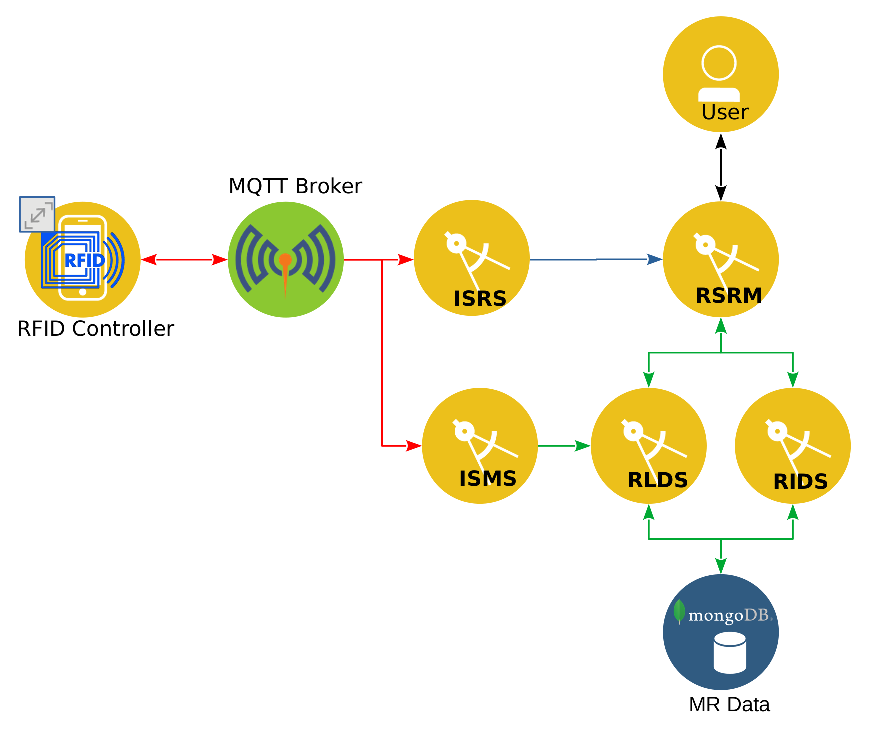
\includegraphics[scale=0.7]{rsms_design.eps}
	\caption{Microservices Components}
	\label{fig:rsms-ms-components}
\end{figure}

\section{System Components}
Three system components that make up this subsystem:
\begin{itemize}
\item \gls{rfid} Controller is a micro-controller that processes \gls{rfid} tags obtained from a \gls{rfid} reader and then publishes \gls{iot} messages to the \gls{mqtt} Broker, one or more micro-controllers can be connected to the network;
\item Network is a \gls{tcpip} communication medium that connects the \gls{rfid} Controller (one or more), \gls{mqtt} Broker and \gls{rsrm} components; and
\item Host is a computer that runs the \gls{mqtt} Broker and other \gls{rsrm} micro-services components.
\end{itemize}

\begin{figure}[H]
	\centering
		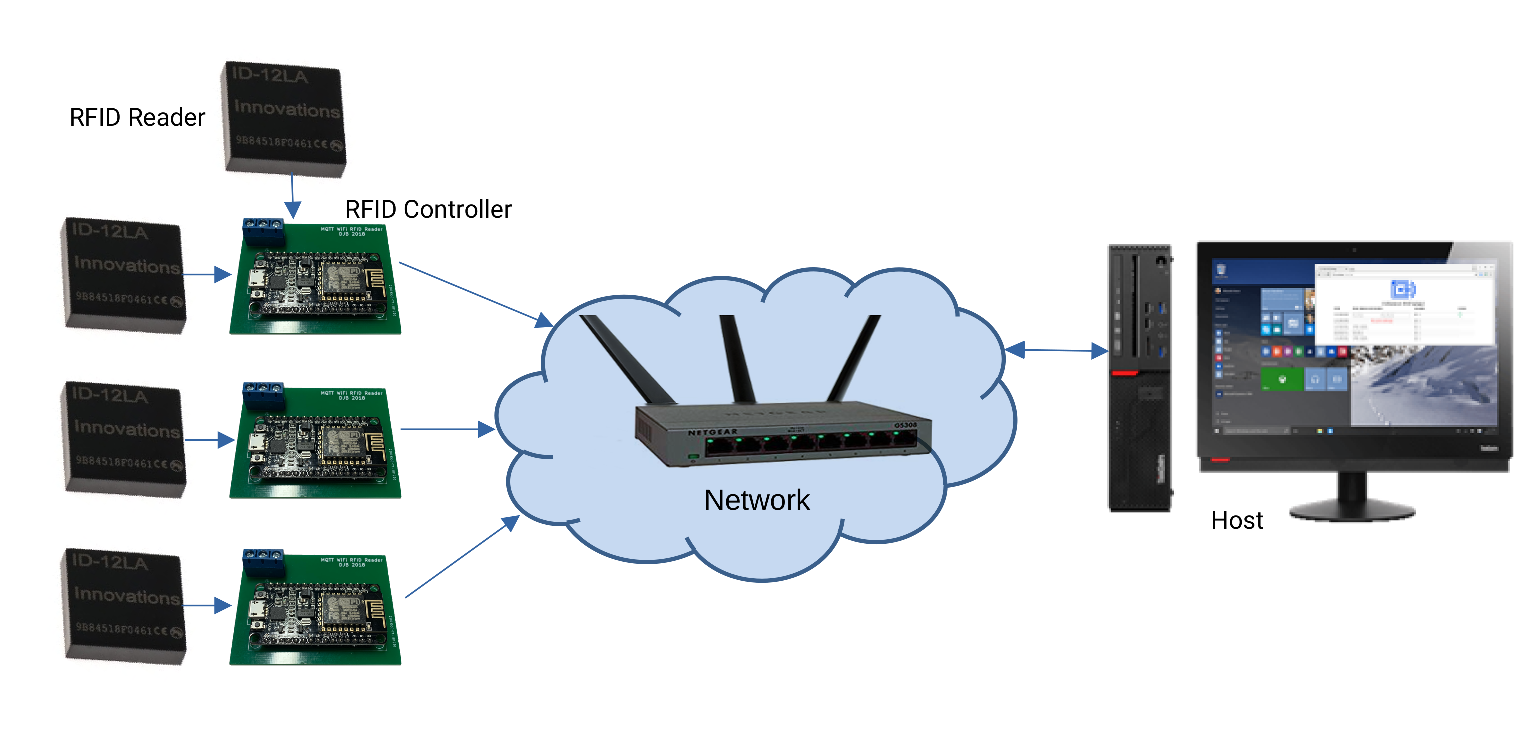
\includegraphics[scale=0.7]{rsms_system.eps}
	\caption{System Components}
	\label{fig:rsms-system-components}
\end{figure}

